\documentclass[tikz,border=3mm]{standalone}
\usepackage[T1]{fontenc}
\usepackage[scaled=0.95]{helvet}
\renewcommand{\familydefault}{\sfdefault}
\usepackage{pgfplots}
\usepackage{xcolor}
\usetikzlibrary{arrows.meta}
\pgfplotsset{compat=1.18}
\definecolor{ink}{HTML}{14213D}
\definecolor{blue}{HTML}{0B5CAD}
\definecolor{rulegrey}{HTML}{C9CED6}
\definecolor{cfull}{HTML}{1F6FB2}
\definecolor{cnover}{HTML}{8DBBE3}
\definecolor{cbzero}{HTML}{E08A2E}
\definecolor{cbone}{HTML}{B5443A}
\definecolor{crev}{HTML}{F2C14E}
\definecolor{good}{HTML}{2E7D4F}
\definecolor{bad}{HTML}{C0392B}
\definecolor{hilite}{HTML}{FFE066}
\definecolor{codebg}{HTML}{1E2329}
\pgfplotsset{poster/.style={font=\sffamily\fontsize{14}{17}\selectfont,
  every axis label/.append style={font=\sffamily\fontsize{15}{18}\selectfont},
  every tick label/.append style={font=\sffamily\fontsize{13}{16}\selectfont},
  major tick length=2mm, axis line style={line width=0.8pt, black!60},
  tick style={black!60}, grid style={black!12,line width=0.6pt}}}
\begin{document}

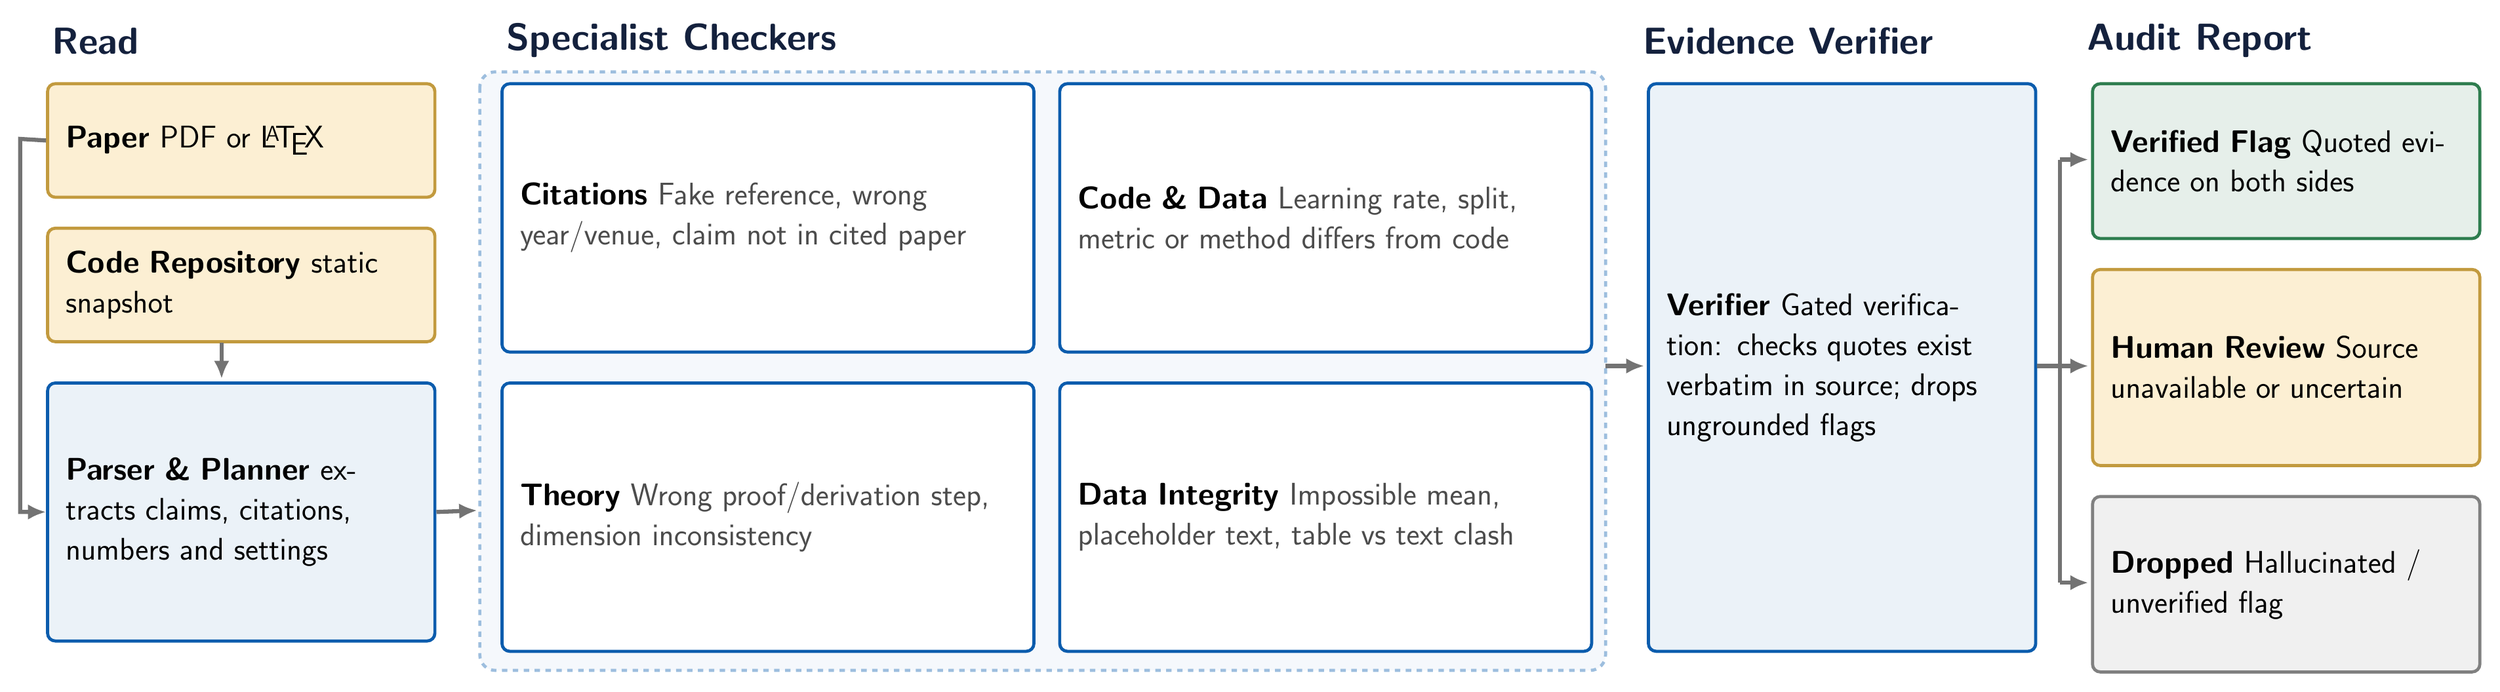
\begin{tikzpicture}[x=1mm, y=1mm, font=\sffamily\fontsize{18}{22}\selectfont,
  bx/.style={draw=#1, line width=0.6mm, rounded corners=1.5mm, align=left, inner xsep=3.5mm,
    inner ysep=2mm, anchor=north west},
  ar/.style={-{Latex[length=3.5mm,width=3mm]}, line width=0.8mm, black!55},
  ln/.style={line width=0.8mm, black!55},
  stitle/.style={anchor=west, font=\sffamily\bfseries\fontsize{22}{26}\selectfont\color{ink}}]
\foreach \x/\n/\s in {0/1/Read, 88/2/Specialist Checkers, 308/3/Evidence Verifier, 394/4/Audit Report} {
  \node[stitle] at (\x,8) {\s};
}
\node[bx=crev!80!black, fill=crev!25, text width=68mm, minimum height=22mm] (pdf) at (0,0)
  {\textbf{Paper}\ PDF or \LaTeX};
\node[bx=crev!80!black, fill=crev!25, text width=68mm, minimum height=22mm] (repo) at (0,-28)
  {\textbf{Code Repository}\ static snapshot};
\node[bx=blue, fill=blue!8, text width=68mm, minimum height=50mm] (parse) at (0,-58)
  {\textbf{Parser \& Planner}\ extracts claims, citations, numbers and settings};
\draw[ar] (34,-50.5) -- (34,-57.5);
\draw[ar] (pdf.west) -- (-5,-11) |- (parse.west);

\fill[blue!4, rounded corners=3mm] (84,2) rectangle (302,-114);
\draw[blue!40, line width=0.6mm, dashed, rounded corners=3mm] (84,2) rectangle (302,-114);
\foreach \x/\y/\name/\what in {
   88/0/Citations/{Fake reference, wrong year/venue, claim not in cited paper},
  196/0/Code \& Data/{Learning rate, split, metric or method differs from code},
   88/-58/Theory/{Wrong proof/derivation step, dimension inconsistency},
  196/-58/Data Integrity/{Impossible mean, placeholder text, table vs text clash}} {
  \node[bx=blue, fill=white, text width=96mm, minimum height=52mm] at (\x,\y)
    {\textbf{\name}\ {\color{black!70}\what}};
}
\draw[ar] (parse.east) -- (83.5,-83);

\node[bx=blue, fill=blue!8, text width=68mm, minimum height=110mm] (ver) at (310,0)
  {\textbf{Verifier}\ Gated verification: checks quotes exist verbatim in source; drops ungrounded flags};
\draw[ar] (302,-55) -- (309.5,-55);

\node[bx=good, fill=good!12, text width=68mm, minimum height=30mm] (ok) at (396,0)
  {\textbf{Verified Flag}\ Quoted evidence on both sides};
\node[bx=crev!80!black, fill=crev!25, text width=68mm, minimum height=38mm] (hum) at (396,-36)
  {\textbf{Human Review}\ Source unavailable or uncertain};
\node[bx=black!50, fill=black!6, text width=68mm, minimum height=34mm] (drop) at (396,-80)
  {\textbf{Dropped}\ Hallucinated / unverified flag};
\draw[ln] (ver.east |- 0,-55) -- (390,-55);
\draw[ln] (390,-15) -- (390,-97);
\foreach \y in {-15,-55,-97} \draw[ar] (390,\y) -- (395.5,\y);
\end{tikzpicture}
\end{document}